\documentclass[kravspec/krav.tex]{subfiles}

\begin{document}

\clearpage
\section{Kommunikationsmodul}
\begin{figure}[H]
    \centering
    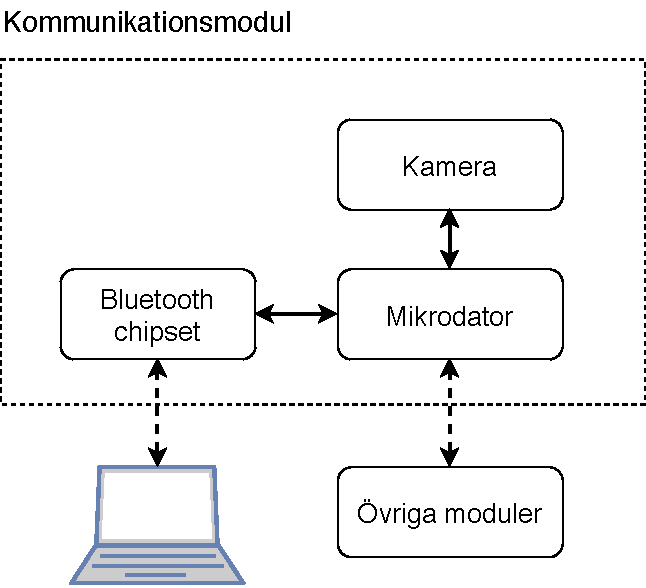
\includegraphics[height=0.4\linewidth]
        {kravspec/figures/kommunikationsmodul.pdf}
    \caption{En möjlig uppsättning av kommunikationsmodulen och dess
    gränssnitt.}
    \label{fig:kommunikationsmodul}
\end{figure}

\subsection{Beskrivning}
Kommunikationsmodulen består av en mikrodator, ett bluetooth chipset samt en
kamera. Kommunikationsmodulen är huvudorganet i systemet och agerar som
dirigent. Modulen kommunicerar med alla andra moduler samt datorn och kopplar
samman dem.

\subsection{Gränssnitt}
Dess uppgift består av bildbearbetning, dirigering av information till andra
moduler samt kommunikation med en dator. Figur \ref{fig:kommunikationsmodul}
visar hur den kan vara kopplad. Till datorn skickas positionen på bilen, avlagd
sträcka, avstånd till vägkant/hinder etc. Dessutom används datorn som
kontroller vid manuell körning av bilen.

\subsection{Krav på kommunikationsmodul}
\begin{reqlist}
    \req{Kommunikationsmodulen skall hantera kommunikation mellan moduler.}
\end{reqlist}

\clearpage
\section{Styrmodul}
\begin{figure}[h]
    \centering
    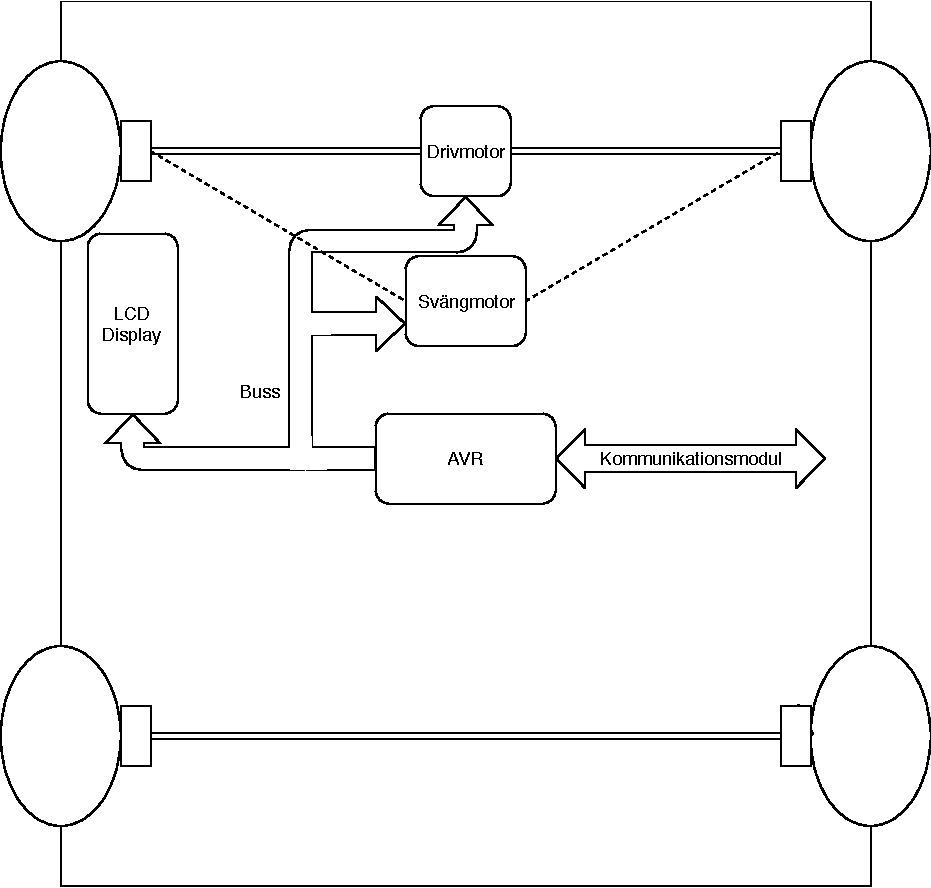
\includegraphics[width=0.6\linewidth]{kravspec/figures/styrmodul.pdf}
    \caption{Ett förslag på hur styrmodulen kan se ut.}
    \label{fig:styrmodul}
\end{figure}

\subsection{Beskrivning}
Styrmodulen består av en kontroller, en drivmotor och en svängmotor som visat i
figur \ref{fig:styrmodul}. Drivmotorn är den motor som gör att bilen rör sig
framåt eller bakåt, medan svängmotorn kontrollererar styraxeln och påverkar
bilens svängradie.

\subsection{Gränssnitt}
Styrmodulen är kopplad till kommunikationsmodulen som ger information om hur
taxins hjul ska bete sig.

\subsection{Krav på styrmodul}
\begin{reqlist}
    \req{Styrmodulen ska sköta direktkommunikationen med bilens motorer utifrån
    kommandon som ges av kommunikationsmodulen.}
    \req{Styrmodulen ska ställa hjulen i rätt position.}
    \req{Styrmodulen ska se till att bilen inte kör av vägen.}
\end{reqlist}

\clearpage
\section{Sensormodul}
\begin{figure}[h]
    \centering
    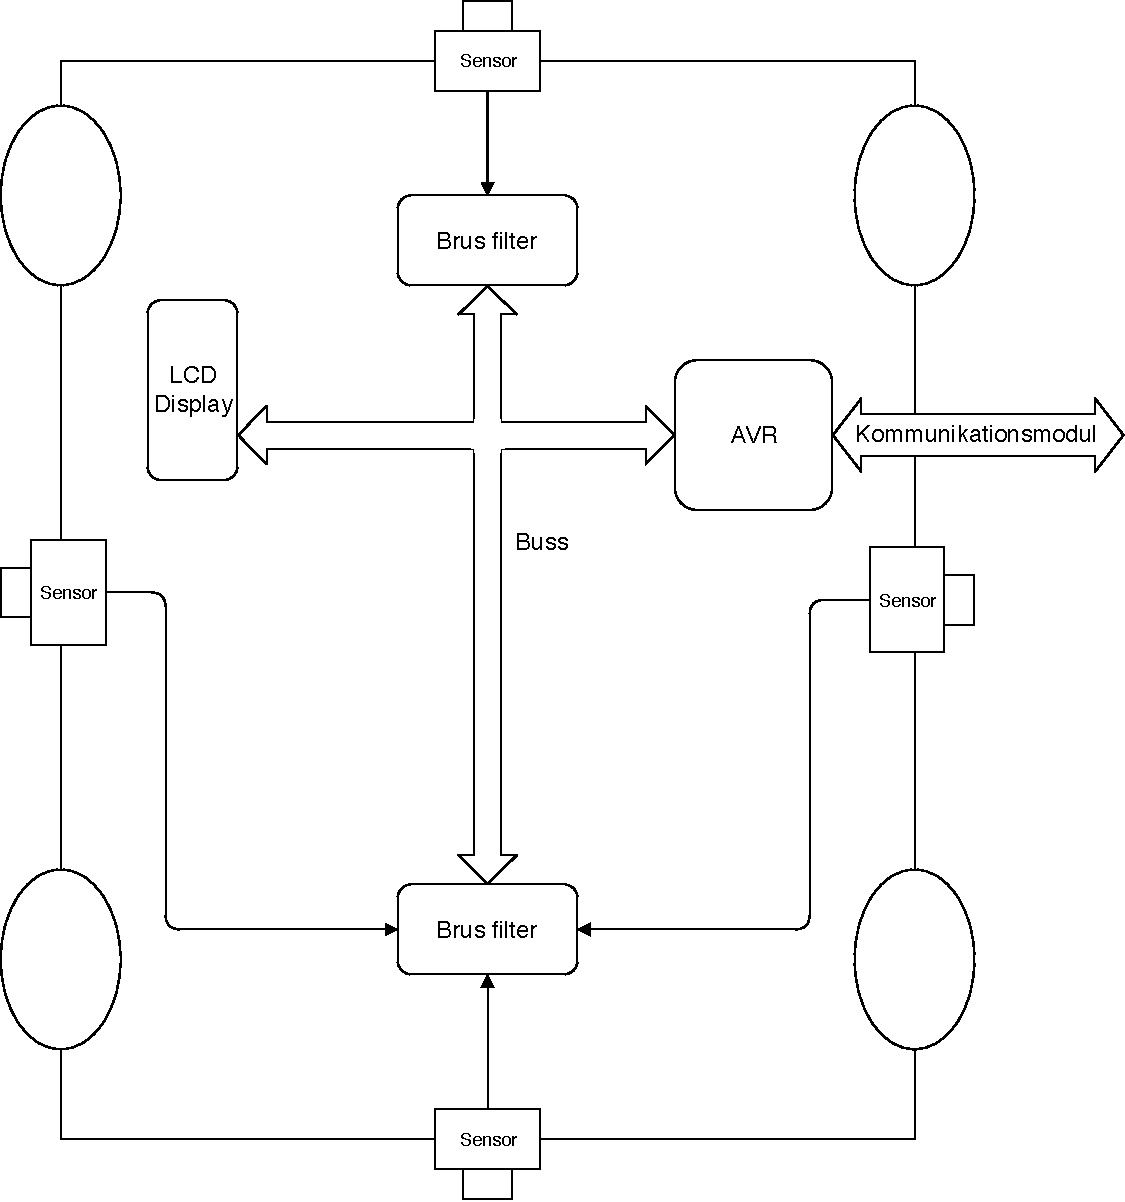
\includegraphics[width=0.6\linewidth]{kravspec/figures/sensormodul.pdf}
    \caption{En möjlig struktur för sensormodulen.}
    \label{fig:sensormodul}
\end{figure}

\subsection{Beskrivning}
Sensormodulen ska bestå av en mikrodator och enhetens sensorer utöver kameran.
Sensorerna skall väljas utefter de krav som behöver uppfyllas. Eventuellt kan
sensormodulen behöva utföra behandling av information innan den skickas till
kontrollmodulen, så att informationen skickas in i SI-enheter.

\subsection{Gränssnitt}
Sensorerna ska vara kopplade till mikrodatorn som behandlar datan och skickar
den vidare till kommunikationsmodulen som kan ses i figur
\ref{fig:sensormodul}.

\subsection{Krav på sensormodul}
\begin{reqlist}
    \req{Sensormodulen ska kunna behandla indata från sensorer och sammanställa
    dessa till ett bestämt gränssnitt.}
    \req{Sensormodulens mikrodator ska ta emot informationen från varje sensor
    och vidarebefodra den till kommunikationsmodulen.}
    \reqspec{original}{2}{En LCD-display på bilen skall visa värden från valda
    sensorer.}
\end{reqlist}

\end{document}
